\PDComment{Based on discussion with Shaz and Cheng, I am trying to do the following: this section will be mostly about the high level overview and how we can model the environment of existing distributed systems and capture all nondeterminism (due to message passing, failures, timers, etc) -- this is not specific to \psharp and thus we could potentially move the \psharp description in the next section and keep this more abstract, but I am not convinced about this. Then the next section is more specifics about \psharp: how the bug-finding runtime works (just overview as its described in our PLDI paper), how the liveness algorithm works, how we handle async/await -- just the generic approach I implemented based on Matt's original work, and maybe some generic discussion about how you can implement extensions of top of \psharp}

Our goal in this work is to \emph{test what is being executed}. Our approach involves using \psharp~\cite{deligiannis2015psharp}, a framework that provides: (i) an \emph{event-driven asynchronous programming} language for developing and modeling distributed systems; and (ii) a \emph{systematic concurrency testing} engine that can systematically explore all interleavings between asynchronous event handlers, as well as other nondeterministic events such as failures and timeouts.

\subsection{The \psharp framework}
\label{sec:method:psharp}

The \psharp language is an extension of \csharp, built on top of Microsoft's Roslyn\footnote{\url{https://github.com/dotnet/roslyn}} compiler, that enables asynchronous programming using communicating state-machines. \psharp machines can interact asynchronously by sending and receiving events,\footnote{We use the word ``event'' and ``message'' interchangeably.} an approach commonly used to develop distributed systems. This programming model is similar to actor-based approaches provided by other asynchronous programming languages (e.g. Scala~\cite{odersky2008programming} and Erlang~\cite{armstrong1996erlang}).

A \psharp machine consists of an input event queue, states, state transitions, event handlers, fields and methods. Machines run concurrently with each other, each executing an event handling loop that dequeues an event from the input queue and handles it by invoking an appropriate event handler. This handler might update a field, create a new machine, or send an event to another machine. In \psharp, a send operation is non-blocking; the message is simply enqueued into the input queue of the target machine, and it is up to the operating system scheduler to decide when to dequeue an event and handle it. All this functionality is provided in a lightweight runtime library, build on top of Microsoft's Task Parallel Library~\cite{leijen2009tpl}.

Because \psharp is built on top of \csharp, the programmer can blend \psharp and \csharp code; this not only lowers the overhead of learning a new language, but also allows \psharp to easily integrate with legacy code. Another advantage is that the programmer can use the familiar programming and debugging environment of Visual Studio.

A key capability of the \psharp runtime is that it can run in \emph{bug-finding mode}, where an embedded systematic testing engine captures and takes control of all sources of nondeterminism (such as event handler interleavings, failures, and client requests) in a \psharp program, and then systematically explores all possible executions to discover bugs.

\psharp is available as open-source\footnote{\url{https://github.com/p-org/PSharp}} and is currently used by various teams in Microsoft to develop and test distributed protocols and systems.

%The \psharp language belongs to the same family of languages as P~\cite{desai2013p}.

\subsection{Overview of our approach}
\label{sec:method:model}

In previous work~\cite{deligiannis2015psharp}, we approached the problem of testing legacy distributed systems as follows. First, we ported the system to \psharp, then we modeled its environment as \psharp state machines, and finally we tested the ported system and its environmental model using the \psharp systematic concurrency testing engine. The limitation of this approach is that it does not allow us to directly test a legacy system, as it has to be re-implemented first in \psharp. However, such endeavor is very costly and time consuming, and thus is not realistic for testing an existing production system, such as the Azure Storage vNext. Also, unless the code under test is the one that will actually execute, there is no guarantee that the real system will be bug-free.

To solve this problem, and allow \psharp to be used for testing legacy distributed systems, we decided to take a different approach. Our approach of testing existing distributed systems using \psharp requires the developer to perform three key modeling tasks:

\begin{enumerate}
\item \psharp operates in the level of communicating state machines, and thus the environment of the system-under-test must be modeled using \psharp machines, while the real components of the system must be wrapped inside \psharp machines. We call this modeled environment the \psharp test harness.

\item The top level asynchrony due to message passing, must be exposed as event sending using the \psharp APIs. If the communication layer is not based on message passing, then additional effort must be spent into refactoring the system to use message passing. This step allows the \psharp runtime to capture and control the nondeterminism due to message passing interleavings during systematic testing.

\item Any other source of nondeterminism in the system or the environment (e.g. failures and timers), must be explicitly modeled using the available \psharp APIs. This would allow \psharp to capture the nondeterminism and control it during systematic testing.
\end{enumerate}

In the remaining of this section, we will use the Azure Storage vNext case study as a running example of how to model a typical distributed system using \psharp. In principle, this modeling methodology is not specific to \psharp but can be used in combination with any systematic testing tool. We decided to use \psharp as it is a mature tool that provides a lot of modeling power via its \csharp language extensions and has an embedded systematic concurrency testing engine inside its runtime.

We argue that our approach is \emph{flexible} since it allows the user to model \emph{as much} or \emph{as little} of the environment as required to achieve the desired level of testing. We also argue that our approach is \emph{generic} since a programmer can build on top of it to test more complicated use cases (see Section~\ref{}). Furthermore, the language features that are required to be used to connect the real code with the modeled code, are already being heavily used in production for testing purposes (e.g. \emph{virtual method dispatch}), which significantly lowers the bar for product groups to embrace \psharp for testing.

In Section~\ref{sec:psharp} we will present more specifics of how the \psharp bug-finding runtime works and extensions that we did since the original work~\cite{deligiannis2015psharp} to be able to use \psharp to systematically test production code.

\subsection{Testing Target}
\label{sec:method:wrap_target}

The testing target in this case is Extent Manager, from the real vNext codebase. It is wrapped inside a \psharp machine in the test setup.

As shown in Figure~\ref{fig:wrap_target}, the \texttt{ExtentManagerMachine} is a wrapper machine and is used to connect the \psharp modeled code with the legacy \csharp code. A typical wrapper machine contains a handle (as a field) to the system component that is being wrapped (in our case the real Extent Manager object) and the event handlers are responsible for translating any received events to method calls in the real code that is being tested. The \texttt{ExtentManager} is accompanied by a mocked version of the real Network Engine class. The real Extent Manager is communicating with the outside world via remote procedure calls, but in \psharp harness we want to capture this communicating and expose it as calls to \psharp communicating primitives. This is discussed in detail in Section~\ref{sec:method:model:dispath}.

\begin{figure}[t]
\begin{lstlisting}
// Wrapping the target vNext component in P#
class ExtentManagerMachine : Machine {
  private ExtentManager extMgr; // target vNext component

  void Init()
  {
    extMgr = new ExtentManager();

    extMgr.netEngine = new MockedNetEngine(); // mock network
    extMgr.SkippingJournal = true; // skip persistence
    extMgr.IsMockingTimer = true;	 // disable internal timer
  }

  [OnEventDoAction(typeof(MessageFromExtentNodeEvent), nameof(DeliverMessageAction))]
	
  private void DeliverMessageAction()
  {
    var msg = (CommandMessage)this.Payload;
    // relay messages from Extent Node to Extent Manager
    extMgr.ProcessSingleMessage(msg);
  }
}
\end{lstlisting}
\vspace{-2mm}
\caption{Wrapping vNext Component in \psharp.}
\label{fig:wrap_target}
%\vspace{-2mm}
\end{figure}

\subsubsection{Relaying Inbound Messages}
\label{sec:method:model:incoming}

Messages from mocked Extent Nodes are delivered to the wrapper \psharp machine as events. The wrapper machine processes such events and relay the corresponding messages to its internal Extent Manager (\emph{extMgr.ProcessSingleMessage}). From the perspective of Extent Manager, these messages are no different from these from real Extent Nodes.

%\subsubsection{Using method dispatch for modeling}
\subsubsection{Proxying Outbound Messages}
\label{sec:method:model:dispath}

Method dispatch is the process of selecting which method, from a set of available methods with the same interface, should be invoked during a program's execution. There are two types of method dispatch: \emph{static}, which is resolved during compilation; and \emph{dynamic}, which is resolved in runtime.  \csharp (and thus \psharp) supports both static and dynamic dispatch, and provide the \texttt{virtual} modifier that can be used to declare a method which can be \emph{overridden} during runtime by an inheriting class. This capability is provided by the common language runtime (CLR) of Microsoft's .NET framework, and is a key feature of \csharp as well as other mainstream object-oriented languages.

Using method dispatch for modeling is straightforward. The system under test exposes a set of APIs as \emph{virtual methods}. The developer can then \emph{override} these APIs and replace them with \emph{mocks} that will execute instead of the original implementations during systematic testing with \psharp.

%\begin{figure}[t]
%\begin{lstlisting}
%// Public interface of the real network engine
%class NetworkEngine {
  %public virtual void SendMessage(Socket s, Message msg);
  %public virtual void EnqueueMessage(Message msg);
%}
%
%// The mocked network engine used during testing
%class MockedNetEngine : NetworkEngine {
  %ExtentManager EM; // Handle to actual system under test
  %MachineId Env; // Handle to modeled environment
  %
  %public MockedNetEngine(ExtentManager em, MachineId env) {
    %this.EM = em;
    %this.Env = env;
  %}
  %
  %public override void SendMessage(Socket s, Message msg) {
    %PSharpRuntime.Send(this.Env, new MsgEvent(), s, msg);
  %}
  %
  %public override void EnqueueMessage(Message msg) {
    %this.EM.ProcessMessage(msg);
  %}
%}
%\end{lstlisting}
%\vspace{-2mm}
%\caption{The mocked network engine used for testing the Azure Storage vNext system.}
%\label{fig:enginecode}
%%\vspace{-2mm}
%\end{figure}

\begin{figure}[t]
\begin{lstlisting}
// network interface in vNext codebase
class NetworkEngine {
  public virtual void SendMessage(Socket s, Message msg);
}

// mocked network for capturing Extent Manager messages
class MockedNetEngine : NetworkEngine {
  public override void SendMessage(Socket s, Message msg) {
    // capture and relay Extent Manager messages
    PSharpRuntime.Send(this.Environment, new MessageFromExtentManagerEvent(), s, msg);
  }
}
\end{lstlisting}
\vspace{-2mm}
\caption{Mocked Network Engine.}
\label{fig:enginecode}
%\vspace{-2mm}
\end{figure}

We now give an example of using dynamic dispatch to model the network engine of an extent manager in the Azure Storage vNext case study (see Figure~\ref{fig:enginecode}). The network engine is responsible for sending to and receiving messages from the various components of the system. During real execution, the network engine uses a custom remote procedure call (RPC) .NET library for communication. For testing, though, it is desirable to replace all calls to this RPC library with \psharp send and receive operations, which can be captured and systematically interleaved to find bugs. We easily achieved this by exposing the original send message operation of the network engine as a virtual method, and then overriding it for testing. In the overridden method, we created a \psharp event and then we wrapped the original message in this event's payload. Then, instead of invoking the RPC library, we invoke the \texttt{PSharpRuntime.Send(...)} method, which asynchronously sends the event (containing the original message) to the target extent node machine.

For mocking the receive operation, we take advantage of the implicit receive of events in \psharp machines. When a extent node machine receives an event, an appropriate event handler is invoked, which extracts the original message from the payload and then handles it accordingly.

\subsection{Mocking Extent Node}
\label{sec:method:mock_en}

The \texttt{ExtentNode} machine is a model (less than 150 lines of code) of the real Extent Node and is responsible for generating synchronization events and sending them to the \texttt{ExtentManager} to test the extent manager's repair logic.

briefly describe mocked repair logic.

briefly describe mocked sync logic

%\begin{figure}[t]
%\begin{lstlisting}
%// Wrapping the target vNext component in P#
%class ExtentNodeMachine : Machine {
  %private ExtentNode.ExtentCenter extCtr; // real vNext component
%
	%[OnEventDoAction(typeof(RepairExtentRequestEvent), nameof(ProcessRepairExtentRequest))]
	%[OnEventDoAction(typeof(DownloadExtentRequestEvent), nameof(ProcessDownloadExtentRequestEvent))]
	%[OnEventDoAction(typeof(DownloadExtentResponseEvent), nameof(ProcessDownloadExtentResponseEvent))]
	%[OnEventDoAction(typeof(TimerTickEvent), nameof(ProcessExtentNodeSyncEvent))]
%
  %void ProcessRepairExtentRequest()
  %{
    %var source = GetRepairSourceMachine(this.Payload);
    %PSharpRuntime.Send(source, new DownloadExtentRequestEvent(), this.Payload);
  %}
%
  %void ProcessDownloadExtentRequestEvent()
  %{
	  %var destination = GetRepairDestinationMachine(this.Payload);
    %var ext_id = GetExtentID(this.Payload);
    %
		%Extent ext;
    %if (extCtr.TryGet(ext_id, out ext))
      %PSharpRuntime.Send(destination, new DownloadExtentResponseEvent(), ext);
  %}
%
  %void ProcessDownloadExtentResponseEvent()
  %{
    %var ext = (Extent)this.Payload;
    %extCtr.AddExtent(ext);
%
    %this.Monitor<RepairMonitor>(new NotifyExtentRepairCompletion(), this.NodeID);
  %}
%
  %void ProcessExtentNodeSyncEvent()
  %{
    %var sync = new ExtentNodeSync(this.NodeID);
    %extCtr.Extents.ForEach(ext =>
      %{
        %var rec = new ExtentRecord(ext.ExtentID, ext.Length, ext.Sealed);
        %sync.ExtentRecs.Add(rec);
      %});
    %PSharpRuntime.Send(this.NameNode, new NameNodeMessageEvent(), sync);
  %}
%}
%\end{lstlisting}
%\vspace{-2mm}
%\caption{Mocked Extent Node.}
%\label{fig:mocked_en}
%%\vspace{-2mm}
%\end{figure}

\begin{figure}[t]
\begin{lstlisting}
// Mocking Extent Node in P#
class ExtentNodeMachine : Machine {
  // use real vNext component whenever appropriate
  private ExtentNode.ExtentCenter extCtr;

  [OnEventDoAction(typeof(RepairExtentRequestEvent), nameof(ProcessRepairExtentRequest))]
  [OnEventDoAction(typeof(TimerTickEvent), nameof(ProcessExtentNodeSync))]

  // extent repair logic
  void ProcessRepairExtentRequest()
  {
    var source = GetRepairSourceMachine(this.Payload);
    PSharpRuntime.Send(source, new DownloadExtentRequestEvent(), this.Payload);
  }
  ...

  // extent node sync logic
  void ProcessExtentNodeSync()
  {
    var sync = new ExtentNodeSync(this.NodeID);
    extCtr.Extents.ForEach(ext =>
      {
        sync.ExtentRecords.Add(new ExtentRecord(ext));
      });
    PSharpRuntime.Send(this.ExtentManagerMachine, new MessageFromExtentNodeEvent(), sync);
  }
}
\end{lstlisting}
\vspace{-2mm}
\caption{Mocked Extent Node.}
\label{fig:mocked_en}
%\vspace{-2mm}
\end{figure}


%\subsection{Modeling the environment}
\subsection{Test Harness}
\label{sec:method:model}

The environment of a distributed system might consist of other distributed systems and services, clients, operating system timers, as well as libraries for networking or other purposes. To be able to systematically test a distributed system, this environment must be modeled and all the interactions between the environment and the system, as well as all the nondeterminism, must be captured and controlled by the \psharp runtime.

%\subsubsection{Creating a test harness using \psharp}
\subsubsection{Orchestrating Machines}
\label{sec:method:model:harness}

\begin{figure}[t]
\centering
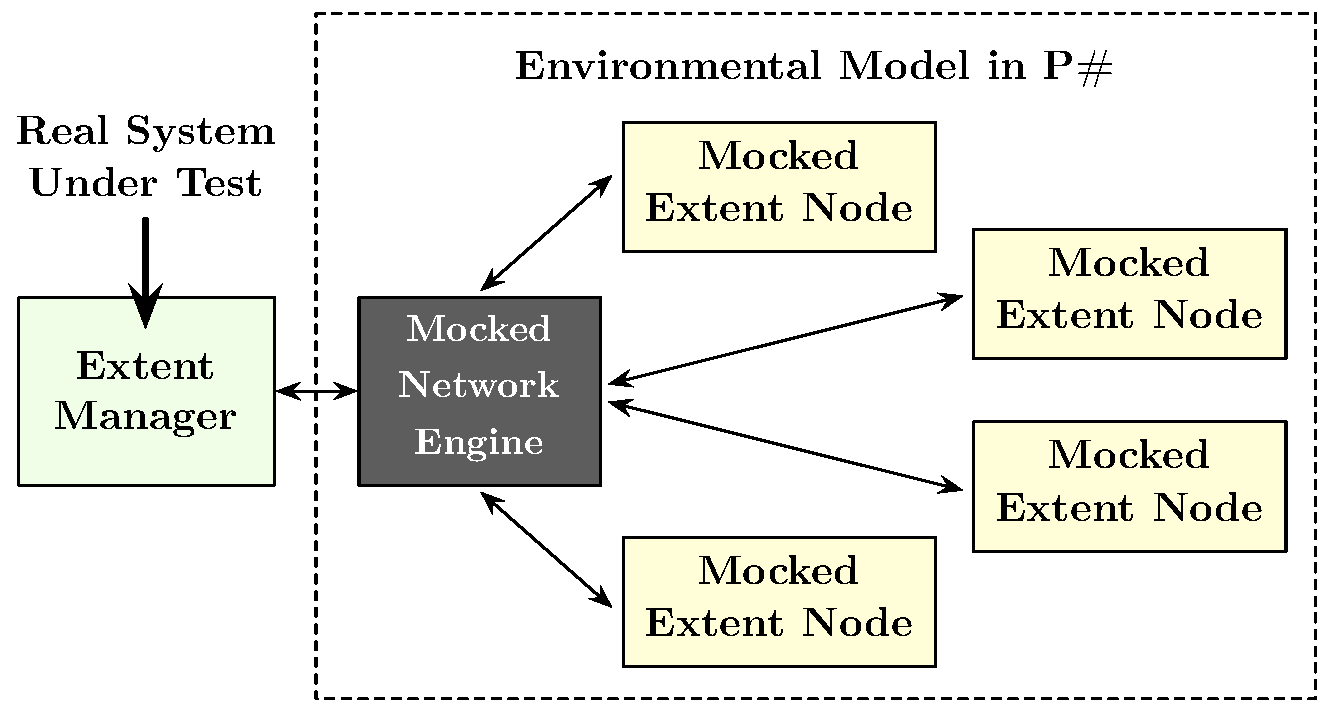
\includegraphics[width=\linewidth]{img/mocked_engine}
\caption{The real environment of the Extent Manager is replaced with a mocked version for testing.}
\label{fig:azurestoremodel}
\end{figure}

Before being able to use \psharp to test an existing distributed system, the environment of the components that the developer wants to test have to be modeled using the \psharp state machine APIs.  This involves creating mock classes that inherit from the \texttt{Machine} abstract class. The \texttt{Machine} class exposes methods for declaring a state machine (e.g. machine states and state transitions) as well as methods for sending events to other machines, declaring event handlers for received events, and accessing the payload from the latest received event.

In the Azure Storage vNext case study, we created the following \psharp machines: \texttt{Environment}, \texttt{ExtentNode}, \texttt{ExtentManager}, and \texttt{Timer}.

The \texttt{Environment} (denoted with a dashed line box in Figure~\ref{fig:azurestoremodel}) is essentially a ``god'' machine: it is the very first machine that is created; has a handle to all other machines in the harness; and includes the logic based on which the test harness will execute. The programmer is free to create either a finite test harness (e.g. with a predefined number of node failures) or an infinite test harness (e.g. with an unbounded number of failures), as long as any nondeterminism (e.g. when to insert a failure) is captured using the available \psharp APIs.

Finally, the \texttt{Timer} machine models the operating system timer and is responsible for triggering events related to the Azure Storage vNext logic (e.g. synchronization messages, heartbeats and repair logic loops). This is discussed in detail in Section~\ref{sec:method:model:timers}.

\subsubsection{Modeling and injecting failures}
\label{sec:method:model:failures}

In production, each Extent Node of the Azure Storage vNext system periodically (every 5 seconds) sends a heartbeat to the Extent Manager which notifies that the Extent Node is alive. Because we want to model failures and systematically inject them using \psharp, we abstract away the heartbeat mechanism in our harness. However, the Extent Manager logic relies on time intervals to detect node failures (see Figure~\ref{fig:expiration}). The way to abstract this time-related logic and connect the real code with the modeled code is to use virtual dispatch and override the virtual \texttt{IsNodeExpired} method with a mocked version.

\begin{figure}[t]
\begin{lstlisting}
// Real code for detecting node expiration
public virtual bool IsNodeExpired(string id, DateTime time)
{
  return DateTime.Compare(time, DateTime.Now) <= 0;
}

// Mocked code for detecting node expiration
public override bool IsNodeExpired(string id, DateTime time)
{
  return this.DeletedNodes.Contains(id);
}
\end{lstlisting}
\vspace{-2mm}
\caption{Abstracting the node expiration logic in the Extent Manager component of Azure Storage vNext.}
\label{fig:expiration}
%\vspace{-2mm}
\end{figure}

Figure~\ref{fig:expiration} presents how we mocked the node expiration detection method. Instead of comparing the time interval as in the original code, we now check if the set \texttt{DeletedNodes} contains the id of the Extent Node that we are checking for expiration. If it contains the id, then it means that the node has failed. The \texttt{Environment} machine that we have created as part of our testing \psharp harness, will nondeterministically choose a node to kill, then send the id of this killed node to the Extent Manager wrapper machine, who will in turn add it to the \texttt{DeletedNodes} set.

\subsubsection{Entry point to a \psharp test harness}
\label{sec:method:model:entrypoint}

A developer can specify the entry point of a \psharp test harness similar to how unit tests are typically written. Figure~\ref{fig:entrypoint} shows the source code of the entry point for the Azure Storage vNext \psharp test harness. The programmer can declare an entry point method using the \texttt{Microsoft.PSharp.Test} attribute. When the \psharp systematic testing engine is invoked, it will scan the binary and attempt to find a static method declared with this attribute. When such a method is found (in our example the \texttt{Execute()} method), the testing engine will invoke it and start testing the program. The systematic engine can optionally run multiple iterations of the test harness, each one potentially exploring a different schedule. In each iteration, the program state will be reset (any static fields must be explicitly reset by the programmer) and the entry point will be re-invoked.

\begin{figure}[t]
\begin{lstlisting}
[Microsoft.PSharp.Test]
public static void Execute()
{
  PSharpRuntime.CreateMachine(typeof(Environment));
}
\end{lstlisting}
\vspace{-2mm}
\caption{Static \csharp method acting as the entry point to the Azure Storage vNext \psharp test harness.}
\label{fig:entrypoint}
%\vspace{-2mm}
\end{figure}

\subsubsection{Abstracting timers}
\label{sec:method:model:timers}

Distributed systems are often using timers to determine when an event should be send from one component to another. For example, in the Azure Storage vNext system, each Extent Node is associated with a timer that fires of a synchronization message every 5 minutes and a heartbeat every 5 seconds. This timer is related to the liveness bug that we discovered: the synchronization message that gets fired every 5 minutes can potentially race with an Extent Node failure; if it arrives after the node failed, then the bug would manifest. Traditional testing techniques cannot easily find such a bug, due to the very infrequent occurrence of this race due to the timer. 

Our methodology in \psharp to systematically test distributed systems that rely on timers, is to abstract timers away, model them using message passing communication and introduce nondeterminism in their firing. This nondeterminism is introduced using the \psharp \texttt{Nondet()} method, which returns a nondeterministic boolean value that is controlled by the \psharp runtime during systematic testing.

Figure~\ref{fig:timer} shows how we modeled a generic timer in the Azure Storage vNext case study. The Extend Manager, as well as each Extent Node in the harness, is associated with a unique \texttt{Timer} machine. When creating this machine, we pass as a payload the id of the machine that owns this timer. When the \texttt{Timer} machine is created, it stores this id in the \texttt{Owner} field and then transitions to the \texttt{Active} state. In this state, the \texttt{Timer} loops infinitely and nondeterministically (using \texttt{Nondet()}) sends a \texttt{TimerTickEvent} to \texttt{this.Owner}. When the Extent Node owner receives this event, it handles it by generating a synchronization message that is being send to the Extent Manager. Similarly, when the Extent Manager receives a \texttt{TimerTickEvent} from its own \texttt{Timer}, it handles it by nondeterministically invoking repair-related methods in the Extent Repair Center data structure. 

\begin{figure}[t]
\begin{lstlisting}
internal class Timer : Machine
{
  MachineId Owner; // Id of the owner machine

  [Start]
  [OnEntry(nameof(InitOnEntryAction))]
  [OnEventGotoState(typeof(Unit), typeof(Active))]
  class Init : MachineState { }

  void InitOnEntryAction()
  {
    this.Owner = (MachineId)this.Payload;
    // triggers state transition to Active
    this.Raise(new Unit());
  }

  [OnEntry(nameof(ProcessTickEvent))]
  [OnEventGotoState(typeof(Unit), typeof(Active))]
  class Active : MachineState { }

  void ProcessTickEvent()
  {
    // Nondeterministic boolean choice controlled by P#
    if (this.Nondet())
      // sends a timer tick event to the owner machine
      this.Send(this.Owner, new TimerTickEvent());
    // triggers state transition to Active
    this.Raise(new Unit());
  }
}
\end{lstlisting}
\vspace{-2mm}
\caption{Timers in Azure Storage vNext are modeled as nondeterministic \psharp machines.}
\label{fig:timer}
%\vspace{-2mm}
\end{figure}
